% Written by src/detection/final_figures.py; needs \usepackage{graphicx} and results/figures/ in \graphicspath.
\begin{figure*}[tb]
  \centering
  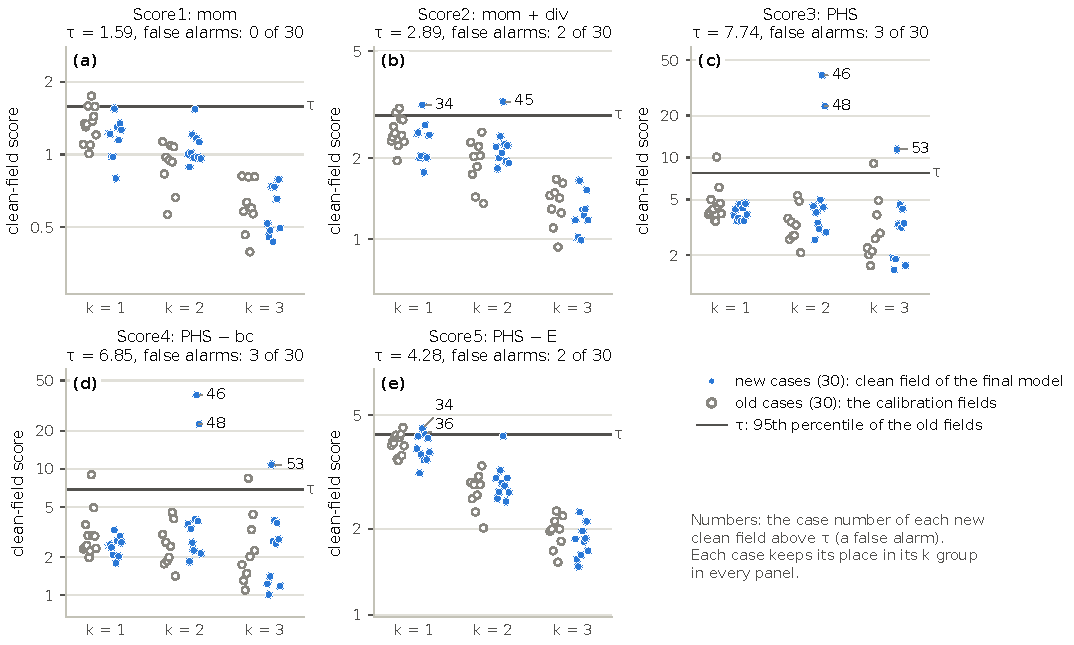
\includegraphics[width=\textwidth]{fig_clean_scores_vs_tau.pdf}
  \caption{The clean field of each of the 30 new cases (filled), and of the 30 old cases the calibration was fitted on (open), for each score and $k$; line: the frozen $\tau$, the 95th percentile of the open points (so 2 of them lie above it). Each new clean field above $\tau$ is a false alarm, labelled with its case number: Score1 none; Score2 case\_34 ($k = 1$) and case\_45 ($k = 2$); Score3 case\_46 ($k = 2$), case\_48 ($k = 2$) and case\_53 ($k = 3$); Score4 case\_46 ($k = 2$), case\_48 ($k = 2$) and case\_53 ($k = 3$); Score5 case\_34 ($k = 1$) and case\_36 ($k = 1$). Score1, Score2 and Score5 score the clean fields of $k = 1$ highest, as the pre-registered protocol expects (Spearman correlation of the clean score with $k$: $-0.80$, $-0.78$ and $-0.90$). Score3 and Score4 flag case\_46, case\_48 and case\_53 instead ($k = 2, 2, 3$), whose normalized energy terms $\bar S_E$ are 36.1, 20.4 and 9.14. $S_E$, the mean squared gap between the kinetic energy and its exact decay, is not scaled by $U_0$, so it grows like $U_0^4$ times the squared relative energy error. These cases have $U_0$ = 1.86, 1.66 and 1.91, and case\_46 and case\_48 have the largest relative energy errors of all 60 models ($\sqrt{S_E}$ over the exact initial energy $U_0^2/4$: 0.84 and 0.79\%, against at most 0.48\% for the old cases).}
  \label{fig:clean_scores_vs_tau}
\end{figure*}
